\chapter{An Introduction to Subgroups and Isomorphisms}
\label{chapter:intro_subgroups_isomorphisms}
\thispagestyle{empty}

In this chapter, we'll continue to utilize our intuitive definition of a group.  That is, a group $G$ is a set of actions that satisfies the following rules.

\begin{description}
\item[Rule 1.] There is a predefined list of actions that never changes.
\item[Rule 2.] Every action is reversible.
\item[Rule 3.] Every action is deterministic.
\item[Rule 4.] Any sequence of consecutive actions is also an action.
\end{description}

In the previous chapter, we constructed lots of Cayley diagrams for various groups.  To construct a Cayley diagram for a group $G$, we need to first identify a set of generators, say $S$.  Recall that our choice of generators is important as changing the generators can result in a different Cayley diagram.  

In the Cayley diagram for $G$ using $S$, all the actions of $G$ are represented by the vertices of the graph.  Each vertex corresponds to a unique action.  This does not imply that there is a unique way to obtain a given action from the generators.  Each of the generators determines an arrow type in the diagram.  One way to distinguish the different arrow types is by using different colors.  An arrow of a particular color always represents the same generator.

One of the vertices in the diagram is labeled by the do-nothing action, often denoted by $e$.  Each of the other vertices are labeled by words that correspond to following arrows (forwards or backwards) from $e$ to a given vertex.  There may be many ways to do this as each sequence of arrows corresponds to a unique word.  So, a vertex could be potentially labeled by many words.  However, we'll often just pick one.  Also, one potentially confusing item is that we read our words from right to left.  That is, the first arrow we follow out of $e$ is the rightmost generator in the word.

\begin{section}{Subgroups}\label{sec:intuitive_subgroups}

\begin{exercise}
Recall the definition of ``subset."  What do you think ``subgroup" means?  Try to come up with a potential definition.  Try not to read any further before doing this.
\end{exercise}

Before continuing, gather up the following Cayley diagrams:
\begin{itemize}
\item $\Spin_{1\times 2}$. There are 3 of these.  I drew one for you in Chapter~\ref{chapter:cayley_diagrams} and you discovered two more in Exercise~\ref{exer:minimal_Cayley_Spin1by2}.
\item $S_2$.  See Exercise~\ref{exer:introducing_S2}.
\item $R_4$.  See Exercise~\ref{exer:introducing_R4}.
\item $D_3$.  There are two of these.  See exercises \ref{exer:introducing_D3} and \ref{exer:alternate_D3}.
\item $D_4$.  See Exercise~\ref{exer:introducing_D4}.
\end{itemize}

\begin{exercise}\label{exer:R4_in_D4}
Examine your Cayley diagrams for $D_4$ and $R_4$.  Make some observations.  How are they similar and how are they different?  Can you reconcile the similarities and differences by thinking about the actions of each group?
\end{exercise}

Hopefully, one of the things you noticed in the previous exercise is that we can ``see" $R_4$ inside of $D_4$ (and hopefully you didn't just read that before completing the exercise).  You may have used different colors in each case and maybe even labeled the vertices with different words, but the overall structure of $R_4$ is there nonetheless.

\begin{exercise}\label{exer:R4_subgroup_D_4}
If you just pay attention to the configuration of arrows, it appears that there are two copies of the Cayley diagram for $R_4$ in the Cayley diagram for $D_4$.  Isolate these two copies by ignoring the edges that correspond to the generator $s$.  Paying close attention to the words that label the vertices from the original Cayley diagram for $D_4$, are either of these groups in their own right?
\end{exercise}

Recall that the do-nothing action must always be one of the actions included in a group.  If this didn't occur to you when doing the previous exercise, you might want to go back and rethink your answer.  Just like in the previous exercise, we can often ``see" smaller groups living inside larger groups.  These smaller groups are called \textbf{subgroups}.

\begin{intuitivedef}
Let $G$ be a group of actions and let $H\subseteq G$.  We say that $H$ is a \textbf{subgroup} if and only if $H$ is a group in its own right.  In this case, we write $H\leq G$.
\end{intuitivedef}

In light of Exercise~\ref{exer:R4_subgroup_D_4}, we would write $R_4\leq D_4$.  The second sub-diagram of $D_4$ that resembles $R_4$ cannot be a subgroup because it does not contain the do-nothing action.  However, since it looks a lot like $R_4$, we call it a \textbf{clone} of $R_4$.

The next theorem\footnote{Perhaps we should call this an ``Intuitive Theorem" since we are using an intuitive definition of a group.} tells us that if we already have a subset of a group, we only need to check two of our rules instead of four.

\begin{theorem}\label{thm:informal_subgroup_criterion}
Let $G$ be a group of actions and let $H\subseteq G$. Then $H$ is a subgroup if and only if $H$ satisfies Rules 2 and 4.%Note: I should probably discuss how the predefined list of generators in Rule 1 is potentially modified.
\end{theorem}

There are a couple subgroups that every group has.

\begin{theorem}\label{thm:trivial_subgroup1}
Let $G$ be a group of actions.  Then $\{e\}\leq G$.
\end{theorem}

\begin{exercise}
Let $G$ be a group and let $e\in G$.  What does the Cayley diagram for the subgroup $\{e\}$ look like?
\end{exercise}

Earlier, we referred to subgroups as being ``smaller."  However, our definition does not imply that this has to be the case.

\begin{theorem}\label{thm:trivial_subgroup2}
Let $G$ be a group of actions.  Then $G\leq G$.
\end{theorem}

We refer to subgroups that are strictly smaller than the whole group as \textbf{proper subgroups}.

Lots of groups have been given formal names (e.g., $D_4$, $R_4$, etc.).  However, not every group or subgroup has a name.  In this case, it's useful to have notation to refer to specific subgroups.

\begin{definition}\label{def:subgroup_gen_by}
Let $G$ be a group of actions and let $g_1,\ldots, g_n$ be distinct actions from $G$.  We define $\langle g_1,\ldots, g_n\rangle$ to be the smallest subgroup containing $g_1,\ldots, g_n$.  In this case, we call $\langle g_1,\ldots, g_n\rangle$ the \textbf{subgroup generated by} $g_1,\ldots, g_n$.
\end{definition}

For example, consider $r, s, s'\in D_3$ (as defined in exercises~\ref{exer:introducing_D3} and \ref{exer:alternate_D3}).  Then $\langle r,s\rangle=\langle s, s'\rangle=D_3$.  Recall that $R_4$ was the subgroup of rotations of the square.  Similarly, the group of rotations of an equilateral triangle is called $R_3$.  Then using the $r$ from $D_3$, we have $\langle r\rangle = R_3$, which is a subgroup of $D_3$.

Note that in Definition~\ref{def:subgroup_gen_by}, we used a finite number of generators.  There's no reason we have to do this.  That is, we can consider groups/subgroups generated by infinitely many elements.

\begin{exercise}
Consider $\Spin_{1\times 2}$.  
\begin{enumerate}
\item[(a)] Can you find the Cayley diagram for $\langle t_1\rangle$ as a subgroup of $\Spin_{1\times 2}$?
\item[(b)] Write down all the actions of the subgroup $\langle t_1, t_2\rangle$. Write them as words in $t_1$ and $t_2$.  Can you find the Cayley diagram for $\langle t_1, t_2\rangle$ as a subgroup of $\Spin_{1\times 2}$?  Can you find a clone for $\langle t_1, t_2\rangle$?
\end{enumerate}
\end{exercise}

One of the benefits of Cayley diagrams is that they are usual for visualizing subgroups.  However, recall that if we change our set of generators, we might get a very different looking Cayley diagram.  The upshot of this is that we may be able to see a subgroup in one Cayley diagram for a given group, but not be able to see if Cayley diagram with a different set of arrows.

\begin{exercise}
We currently have two different Cayley diagrams for $D_3$ (see exercises \ref{exer:introducing_D3} and \ref{exer:alternate_D3}).  
\begin{enumerate}
\item[(a)] Can you find the Cayley diagram for $\langle e\rangle$ as a subgroup of $D_3$?  Can you see it in both Cayley diagrams for $D_3$?  Can you find all the clones?
\item[(b)] Can you find the Cayley diagram for $\langle r\rangle =R_3$ as a subgroup of $D_3$?  Can you see it in both Cayley diagrams?  Can you find all the clones?
\item[(c)] Find the Cayley diagrams for $\langle s\rangle$ and $\langle s'\rangle$ as subgroups of $D_3$.  Can you see them in both Cayley diagrams for $D_3$?  Can you find all the clones?
\end{enumerate}
\end{exercise}

\begin{exercise}\label{exer:subgroups_D4}
Consider $D_4$.  Let $h$ be the action that reflects (i.e., flips over) the square over the horizontal midline and let $v$ be the action that reflects the square over the vertical midline.  Also, we'll use $r^2$ as shorthand for the action $rr$ that does $r$ twice in a row.  Which of the following are subgroups of $D_4$?  In each case, justify your answer.  If a subset is a subgroup, try to find a minimal set of generators.  Also, determine whether you can see the subgroups in our Cayley diagram for $D_4$.
\begin{enumerate}
\item[(a)] $\{e, r^2\}$
\item[(b)] $\{e,h\}$
\item[(c)] $\{e, h, v\}$
\item[(d)] $\{e, h, v, r^2\}$
\end{enumerate}
\end{exercise}

The last subgroup above is often referred to as the \textbf{Klein four-group} and is denoted by $V_4$.

Let's introduce a group we haven't seen yet.  We define the \textbf{quaternion group} to be the group $Q_8=\{1,-1,i,-i,j,-j,k,-k\}$ having the following Cayley diagram with generators $i, j, -1$.  In this case, 1 is the do-nothing action.

\tikzstyle{vert} = [circle, draw, fill=grey,inner sep=0pt, minimum size=6mm]
\tikzstyle{b} = [draw,very thick,blue,-stealth]
\tikzstyle{r} = [draw, very thick, red,-stealth]
\tikzstyle{g} = [draw, very thick, green, stealth-stealth]

\begin{center}
\begin{tikzpicture}[scale=1.5,auto]
\node (1) at (135:2) [vert] {{\scriptsize $1$}};
\node (i) at (45:2) [vert] {\scriptsize {$i$}};
\node (k) at (-45:2) [vert] {{\scriptsize $k$}};
\node (j) at (-135:2) [vert] {{\scriptsize $j$}};
\node (-1) at (135:1) [vert] {{\scriptsize $-1$}};
\node (-i) at (45:1) [vert] {{\scriptsize $-i$}};
\node (-k) at (-45:1) [vert] {{\scriptsize $-k$}};
\node (-j) at (-135:1) [vert] {{\scriptsize $-j$}};

\path[b] (1) to (i);
\path[b] (i) to (-1);
\path[b] (-1) to (-i);
\path[b] (-i) to (1);

\path[b] (-j) to (-k);
\path[b] (-k) to (j);
\path[b] (j) to (k);
\path[b] (k) to (-j);

\path[r] (-k) to (-i);
\path[r] (-i) to (k);
\path[r] (k) to (i);
\path[r] (i) to (-k);

\path[r] (1) to (j);
\path[r] (j) to (-1);
\path[r] (-1) to (-j);
\path[r] (-j) to (1);

\path[g] (1) to (-1);
\path[g] (j) to (-j);
\path[g] (i) to (-i);
\path[g] (k) to (-k);

\end{tikzpicture}
\end{center}

Notice that I didn't mention what the actions actually do.  For now, let's not worry about that.  The relationship between the arrows and vertices tells us everything we need to know.  Also, let's take it for granted that $Q_8$ actually is a group.

\begin{exercise}
Consider $Q_8$.
\begin{enumerate}
\item[(a)] Which arrows correspond to which generators in our Cayley diagram for $Q_8$?
\item[(b)] What is $i^2$ equal to?  That is, what element of $\{1,-1,i,-i,j,-j,k,-k\}$ is $i^2$ equal to?  How about $i^3$, $i^4$, and $i^5$?
\item[(c)] What are $j^2$, $j^3$, $j^4$, and $j^5$ equal to?
\item[(d)] What is $(-1)^2$ equal to?
\item[(e)] What is $ij$ equal to?  How about $ji$?
\item[(f)] Can you determine what $k^2$ and $ik$ are equal to?
\item[(g)] Can you identify a generating set consisting of only two elements?  Can you find more than one?
\item[(h)] What subgroups of $Q_8$ can you see in the Cayley diagram (with generators $i, j, -1$)?
\item[(i)] Find a subgroup of $Q_8$ that you cannot see in the Cayley diagram.
\end{enumerate}
\end{exercise}

\end{section}

\begin{section}{Isomorphisms}

By now you've probably seen enough examples of Cayley diagrams to witness some patterns appearing over and over again.  For example, you've seen chunks of Cayley diagrams that resemble the Cayley diagram for $S_2$ with generator $s$.

\tikzstyle{vert} = [circle, draw, fill=grey,inner sep=0pt, minimum size=6mm]
\tikzstyle{twoway} = [draw, very thick, blue, stealth-stealth]

\begin{center}
\begin{tikzpicture}[scale=1.5,auto]
\node (e) at (0,0) [vert] {{\scriptsize $e$}};
\node (s) at (2,0) [vert] {\scriptsize {$s$}};
\path[twoway] (e) to (s);
\end{tikzpicture}
\end{center}

\noindent Recall that $S_2$ is the group that acts on two coins by swapping their positions.  In this case, $s$ is the action that swaps the left and right coins and $e$ is the do-nothing action.  

If you look at any of the versions of the Cayley diagrams for $\Spin_{1\times 2}$, $D_3$, $D_4$, and $Q_8$ that we've seen, it is easy to identify the portions that ``look like" $S_2$.  For example, if you isolate the Cayley diagram for the subgroup $\langle -1\rangle=\{1,-1\}$ in $Q_8$, we see that it looks just like the Cayley diagram for $S_2$, except the labels are not identical.  The clones of the subgroup $\langle -1\rangle=\{1,-1\}$ in $Q_8$ look like $S_2$, as well, but they do not contain the do-nothing action.  

The one thing that is different about the Cayley diagram for $S_2$ and the Cayley diagram for $\langle -1\rangle$ is that the labels are different.  If we set the Cayley diagram for $S_2$ on top of the Cayley diagram for $\langle -1\rangle$ such that the do-nothing actions match up, then $s$ and $-1$ would correspond to each other.  In other words, the two Cayley diagrams are identical up to relabeling the vertices.

In this case, we say that $S_2$ and the subgroup $\langle -1\rangle$ of $Q_8$ are \textbf{isomorphic} under the correspondence $e\leftrightarrow 1$ and $s\leftrightarrow -1$.  This one-to-one correspondence between the two groups is called an \textbf{isomorphism}, which is depicted in Figure~\ref{fig:isoS2}.
  
\begin{figure}\label{fig:isoS2}
\begin{center}
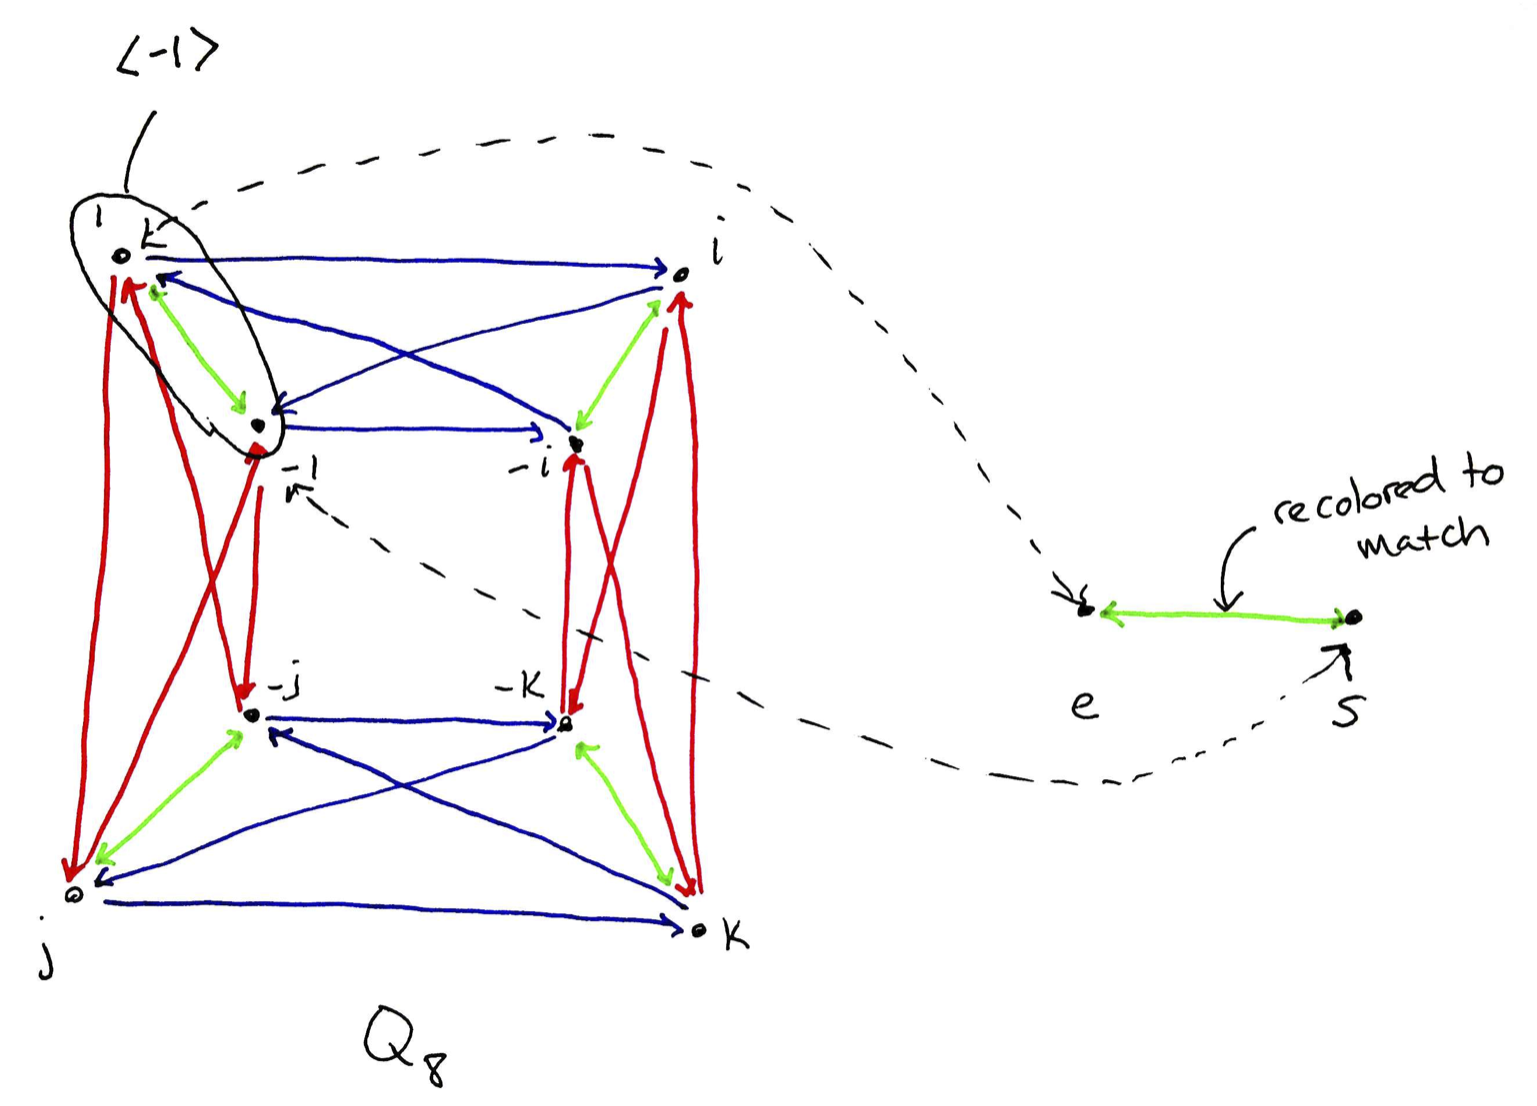
\includegraphics[width=5in]{isoS2.png}
\end{center}
\caption{Isomorphism between $\langle -1\rangle\leq Q_8$ and $S_2$.}
\end{figure}

What this means is that these two groups have the same structure and characteristics.  Or, in other words, these two groups essentially do the ``same kind" of thing.  Clearly, the two do-nothing actions behave the same way.  Also, $s$ and $-1$ both have the property that doing the action twice results in having done nothing (i.e., each element is its own reverse).  Since there are only two elements, there isn't anything else to check.  In groups with more elements, things can get much more complicated.  

It is important to point out that $S_2$ and $\langle -1\rangle$ (in $Q_8$) are not equal.  But they have the same structure.  Identifying when two groups have the same structure (i.e., isomorphic) is an important pursuit in group theory.

If you look at the original Cayley diagram for $\Spin_{1\times 2}$ (with generators $s, t_1, t_2$), we can see three subgroups that look like $S_2$; namely $\langle s\rangle$, $\langle t_1\rangle$, and $\langle t_2\rangle$.  Each of these three subgroups is isomorphic to $S_2$.  

There is one serious potential for confusion here.  Notice that there is an $s$ in $S_2$ and an $s$ in $\Spin_{1\times 2}$.  Despite having identical names, they are not the same element.  Since we only have 26 letters in our alphabet this sort of thing is unavoidable.  Under the isomorphism between $S_2$ and the subgroup $\langle s\rangle$ in $\Spin_{1\times 2}$, the two elements with the same name match up.  That is, these two elements are the ones in each group with the same behavior.

\begin{exercise}
Can you find any other subgroups or groups that are isomorphic to $S_2$?
\end{exercise}

Let's write down an official definition of isomorphic.

\begin{definition}
Let $G$ and $G'$ be two groups.  We say that $G$ and $G'$ are \textbf{isomorphic} if there exist generating sets $S$ and $S'$ for $G$ and $G'$, respectively, such that the corresponding Cayley diagrams are identical where we ignore the labels on the vertices and recolor the edges if necessary.  In this case, we write $G\cong G'$.  Otherwise, we say that $G$ and $G'$ are not isomorphic.  If $G$ and $G'$ are isomorphic, then the one-to-one correspondence determined by matching up the corresponding generators and respecting arrow paths is called an \textbf{isomorphism}.
\end{definition}

The last sentence in the definition above might be a bit much to handle at the moment, but as we construct more examples, the concept should become clear.  The general idea is to take two identical Cayley diagrams (ignoring labels) for $G$ and $G'$ and then set one on top of the other so that the vertices and arrows of the same color match up.  This should be done so that the do-nothing actions correspond to each other.  Then it becomes clear which actions in $G$ correspond to which actions in $G'$.  There might be many ways to do this.

Consider the group $R_4$ with generator $r$ (rotation by $90^\circ$ clockwise).  Now, take a look at the Cayley diagram for $Q_8$ with generators $i, j, -1$.  It should be easy to convince yourself that $R_4$ is isomorphic to both $\langle i\rangle=\{1,i,-i,-1\}$ and $\langle j\rangle=\{1,j,-j,-1\}$.  However, you have to do some rearranging of one of the diagrams to set one on top of the other.  Let's just focus on $\langle i\rangle$.  

How do $R_4$ and $\langle i\rangle$ match up?  We want to pair elements in each group with an element in the other group that has the same behavior.  Clearly, $e$ and $1$ match up since these are the two do-nothing actions.  Also, the reason why we noticed these two groups were isomorphic is because their Cayley diagrams looked the same.  Since each Cayley diagram only had one arrow type determined by $r$ and $i$, we should pair these two elements.  Now, following the arrows around the diagram, we see that $r^2$ must pair with $i^2=-1$ and $r^3$ corresponds to $i^3=-i$.  In summary, the isomorphism between $R_4$ and $\langle i\rangle$ (in $Q_8$) is given by $e\leftrightarrow 1$, $r\leftrightarrow i$, $r^2\leftrightarrow -1$, and $r^3\leftrightarrow -i$ (See Figure~\ref{fig:isoR4}).  You should take a moment to convince yourself that the elements that correspond to each other really do behave in similar ways.

\begin{figure}\label{fig:isoR4}
\begin{center}
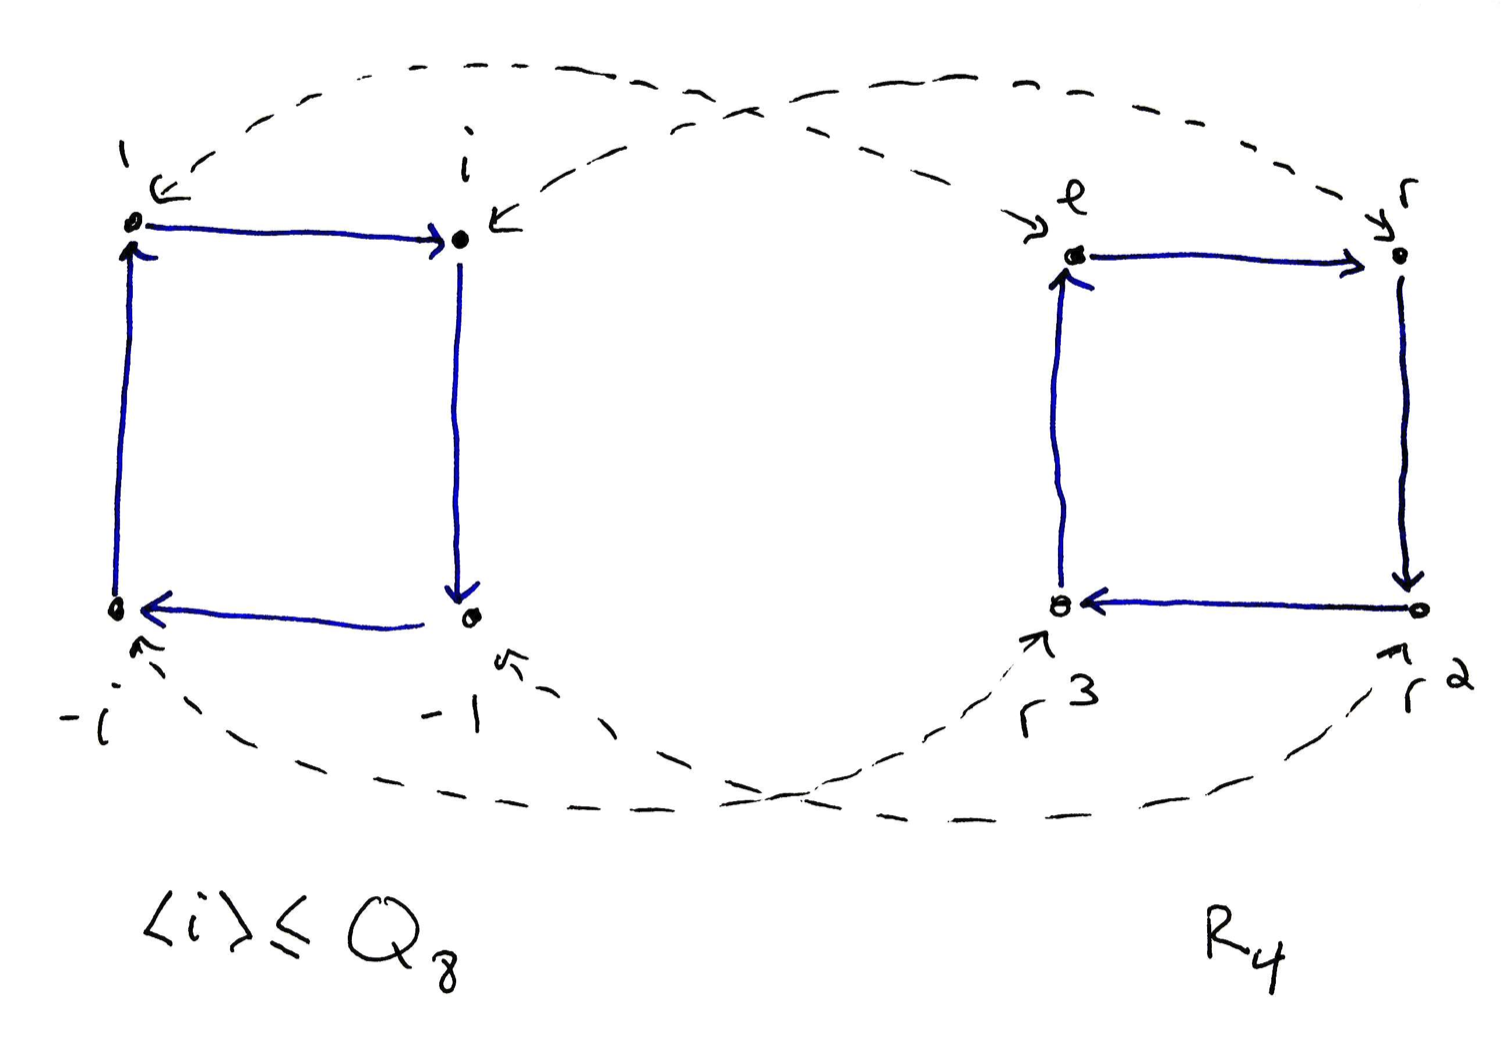
\includegraphics[width=4in]{isoR4.png}
\end{center}
\caption{Isomorphism between $\langle i\rangle\leq Q_8$ and $R_4$.}
\end{figure}

Now, take a look at the Cayley diagram for $D_4$ with generators $r$ and $s$.  As we noticed in Exercise~\ref{exer:R4_in_D4}, $R_4$ is a subgroup of $D_4$.  We could say that this subgroup is isomorphic to $R_4$, but in this case, we can say something even stronger: they are equal!

It turns out that there is a fancy word for the size of a group.

\begin{definition}
If $G$ is a group with $n$ distinct actions, then we say that $G$ has \textbf{order} $n$ and write $|G|=n$.  If $G$ contains infinitely many elements, then we say $G$ has infinite order and write $|G|=\infty$.
\end{definition}

\begin{exercise}
Find the orders of the following groups: $S_2$, $\Spin_{1\times 3}$, $\Spin_{3\times 3}$, $R_4$, $D_3$, $D_4$, $V_4$ (see the comment following Exercise~\ref{exer:subgroups_D4}), and $Q_8$.
\end{exercise}

\begin{theorem}\label{thm:iso_same_order}
Suppose $G$ and $G'$ are two groups of actions such that $G\cong G'$.  Then $|G|=|G'|$.
\end{theorem}

Unfortunately, the converse of the previous theorem is not true in general.  That is, two groups that have the same order may or may not be isomorphic.  

Loosely speaking, if one group has a property that the other does not have, then the two groups cannot be isomorphic.  For example, if one group has the property that every pair of actions commutes (i.e., the order\footnote{Don't confuse the word ``order" in this sentence with the order of a group.} of the actions does not matter), but another group has a pair of actions that do not commute, then the two groups cannot be isomorphic.  Moreover, if one group contains an action that requires a minimum of $k$ applications to get back to the do-nothing action, but a second group does not have such an element, then the two groups cannot be isomorphic.  

Justifying these two claims takes a bit of work and for now, we'll put that on hold.  For the time being, if you don't see why these claims about when two groups are not isomorphic are true, just take them on faith and we will return to the issue in a later chapter.  Feel free to use these ideas in the exercises that follow.

Let's do a bit more exploring.

\begin{exercise}
Using $h$ and $v$ as generators, draw the Cayley diagram for $V_4$.
\end{exercise}

Notice that our standard Cayley diagram for $R_4$ does not look like the Cayley diagram that you just constructed for $V_4$.  This does \emph{not} imply that these two groups are not isomorphic.

\begin{problem}
Determine whether $R_4$ and $V_4$ are isomorphic.  Justify your answer.  If they are isomorphic, specify the isomorphism by listing the correspondence of elements.
\end{problem}

\begin{problem}\label{prob:R6_not_iso_D3}
Consider the group given by the Cayley diagram in Exercise~\ref{exer:intro_R6}.  Let's assume that this is the rotation group for a regular hexagon---called $R_6$.  Determine whether $R_6$ and $D_3$ are isomorphic.  Justify your answer.  If they are isomorphic, specify the isomorphism by listing the correspondence of elements.
\end{problem}

\begin{exercise}
Consider two light switches on a wall side by side.  Consider the group of actions that consists of all possible actions that you can do to the two light switches.  For example, one action is toggle the left light switch while leaving the right alone.  Let's call this group $L_2$.
\begin{enumerate}
\item[(a)] How many distinct actions does $L_2$ have?
\item[(b)] Can you find a minimal generating set for $L_2$?  If so, give these actions names and then write all of the actions of $L_2$ as words in your generator(s).
\item[(c)] Using your generators from part (b), draw a Cayley diagram for $L_2$.
\end{enumerate}
\end{exercise}

\begin{problem}
Determine whether $L_2$ and $V_4$ are isomorphic.  Justify your answer.  If they are isomorphic, specify the isomorphism by listing the correspondence of elements.
\end{problem}

\begin{problem}
Determine whether $Q_8$ and $D_4$ are isomorphic.  Justify your answer.  If they are isomorphic, specify the isomorphism by listing the correspondence of elements.
\end{problem}

\begin{problem}
Determine whether $\Spin_{1\times 2}$ and $D_4$ are isomorphic.  Justify your answer.  If they are isomorphic, specify the isomorphism by listing the correspondence of elements.
\end{problem}

\begin{exercise}
Consider the group that acts on three coins that are in a row by rearranging their positions (but not flipping them over).  This group is called $S_3$.  Numbering the positions of the coins (not the coins themselves) 1, 2, 3 from left to right.  Let $s_1$ be the action that swaps the coins in positions 1 and 2.  Similarly, let $s_2$ be the action that swaps coins in positions 2 and 3.
\begin{enumerate}
\item[(a)] The group $S_3$ consists of 6 actions, which we can generate with $s_1$ and $s_2$.  Write all 6 actions as words in $s_1$ and $s_2$.
\item[(b)] Using $s_1$ and $s_2$ as generators, draw a Cayley diagram for $S_3$.
\end{enumerate}
\end{exercise}

\begin{problem}\label{prob:D3_iso_S3}
Determine whether $S_3$ and $D_3$ are isomorphic.  Justify your answer.  If they are isomorphic, specify the isomorphism by listing the correspondence of elements.  Don't forget that we've drawn two different Cayley diagrams for $D_3$.
\end{problem}

\end{section}